%                      Code_Saturne version 1.3
%                      ------------------------
%
%     This file is part of the Code_Saturne Kernel, element of the
%     Code_Saturne CFD tool.
%
%     Copyright (C) 1998-2008 EDF S.A., France
%
%     contact: saturne-support@edf.fr
%
%     The Code_Saturne Kernel is free software; you can redistribute it
%     and/or modify it under the terms of the GNU General Public License
%     as published by the Free Software Foundation; either version 2 of
%     the License, or (at your option) any later version.
%
%     The Code_Saturne Kernel is distributed in the hope that it will be
%     useful, but WITHOUT ANY WARRANTY; without even the implied warranty
%     of MERCHANTABILITY or FITNESS FOR A PARTICULAR PURPOSE.  See the
%     GNU General Public License for more details.
%
%     You should have received a copy of the GNU General Public License
%     along with the Code_Saturne Kernel; if not, write to the
%     Free Software Foundation, Inc.,
%     51 Franklin St, Fifth Floor,
%     Boston, MA  02110-1301  USA
%
%-----------------------------------------------------------------------
%

\programme{clptur}

\vspace{1cm}
%%%%%%%%%%%%%%%%%%%%%%%%%%%%%%%%%%
%%%%%%%%%%%%%%%%%%%%%%%%%%%%%%%%%%
\section{Fonction}
%%%%%%%%%%%%%%%%%%%%%%%%%%%%%%%%%%
%%%%%%%%%%%%%%%%%%%%%%%%%%%%%%%%%%
Ce sous-programme est d\'edi\'e au calcul des conditions aux limites en paroi.
On utilise le formalisme introduit dans \var{CONDLI} pour les conditions
aux limites g\'en\'erales.

Par conditions aux limites en paroi, on entend ici l'ensemble des conditions aux
limites pour la vitesse, les grandeurs turbulentes ($k$, $\varepsilon$,
$R_{ij}$), la temp\'erature lorsqu'elle a une valeur de paroi impos\'ee
(ou l'enthalpie et plus g\'en\'eralement les
{\it VarScalaires}\footnote{Comme dans \fort{condli}, on d\'esignera ici par
{\it VarScalaire} toute variable solution
d'une \'equation de convection-diffusion autre que la
vitesse, la pression et les grandeurs turbulentes $k$, $\varepsilon$ et
$R_{ij}$. La d\'enomination {\it VarScalaire} pourra en particulier se rapporter
\`a la temp\'erature, \`a l'enthalpie ou \`a un scalaire passif.}
\`a traiter en paroi en prenant en compte une loi de similitude
pour la couche limite associ\'ee). Pour les {\it VarScalaires}, en particulier,
lorsque les conditions aux limites de paroi sont du type Neumann (homog\`ene ou non),
elles sont trait\'ees dans \fort{condli} et on ne s'y int\'eresse donc pas
ici. En particulier, les conditions aux limites des  {\it VarScalaires}
repr\'esentant la variance de fluctuations d'autres  {\it VarScalaires} ne
sont pas trait\'ees ici car leur traitement en paroi est de type Neumann homog\`ene.

On indique comment sont calcul\'es les couples de coefficients
$A_b$ et $B_b$ qui sont utilis\'es pour le calcul de certains
termes discrets des \'equations \`a r\'esoudre et qui
permettent  en particulier de d\'eterminer une valeur associ\'ee aux faces
de bord $f_{b,int}$ (en un point localis\'e au ``centre'' de la face de bord,
barycentre de ses sommets) par la
relation $f_{b,int} = A_b+B_b\,f_{I'}$ ($f_{I'}$ est la valeur de
la variable au point
$I'$, projet\'e du centre de la cellule jouxtant le bord sur la droite
normale \`a
la face de bord et passant par son centre~: voir la figure~\ref{Base_Clptur_fig_flux_clptur}).

\begin{figure}[h]
\centerline{\includegraphics[height=7cm]{\repgraphics/fluxbord}}
\caption{\label{Base_Clptur_fig_flux_clptur}Cellule de bord.}
\end{figure}

%%%%%%%%%%%%%%%%%%%%%%%%%%%%%%%%%%
%%%%%%%%%%%%%%%%%%%%%%%%%%%%%%%%%%
\section{Discr\'etisation}
%%%%%%%%%%%%%%%%%%%%%%%%%%%%%%%%%%
%%%%%%%%%%%%%%%%%%%%%%%%%%%%%%%%%%

\etape{Notations\vspace{0,3cm}}
%%%%%%%%%%%%%%%%%%%%%%%%%%%%%%%%%%%%%%%%%%%%%%%%%%%%%%%%%%%%%%%%%%%%%%%%%%%%%%%
La vitesse de la paroi est not\'ee
$\vect{v}_p$. On la suppose projet\'ee dans le plan tangent \`a la paroi (si
elle ne l'est pas, le code la projette).

La vitesse du fluide est not\'ee $\vect{u}$. L'indice $I$, $I'$ ou $F$ d\'esigne le
point auquel elle est estim\'ee. La composante tangentielle par rapport \`a la
paroi est not\'ee $u_\tau$.
 La vitesse du fluide dans le rep\`ere li\'e \`a la paroi (vitesse
``relative'') est not\'ee $\vect{u}^r=\vect{u} - \vect{v}_p$.

Le rep\`ere orthonorm\'e li\'e \`a la paroi est not\'e
$\hat {\mathcal R}=(\vect{\tau},\vect{\tilde{n}},\vect{b})$.
\begin{itemize}
\item [$\bullet$] $\vect{\tilde{n}}=-\vect{n}$ est le vecteur norm\'e
orthogonal \`a la paroi et dirig\'e vers l'int\'erieur du domaine de calcul.
\item [$\bullet$] $\vect{\tau} = \displaystyle\frac{1}{\|\vect{u}^r_{I'}-(\vect{u}^r_{I'}\,.\,\vect{\tilde{n}})\|}\left[\vect{u}^r_{I'}-(\vect{u}^r_{I'}\,.\,\vect{\tilde{n}})\right]$ est le vecteur norm\'e port\'e par la projection de la vitesse
relative en $I'$, $\vect{u}^r_{I'}$, dans le plan tangent \`a la
paroi ({\it i.e.} orthogonal \`a $\vect{\tilde{n}}$)~: voir la
figure~\ref{Base_Clptur_fig_flux_clptur}.
\item [$\bullet$] $\vect{b}$ est le vecteur norm\'e compl\'etant le rep\`ere direct.
\end{itemize}
\vspace{0.2cm}

La distance adimensionnelle limite s�parant la sous-couche visqueuse de la zone
logarithmique est not�e $y^+_{lim}$. Elle vaut $1/\kappa$ (avec $\kappa = 0,42$)
en g�n�ral (valeur de continuit� du gradient de vitesse) et 10,88 en LES (valeur
de continuit� de la vitesse).

Dans le cas du {\bf mod\`ele \`a deux  \'echelles de vitesse},
\begin{itemize}
\item [-] on note $u_k$ la
vitesse de frottement en paroi obtenue \`a partir de l'\'energie turbulente.
On note $u^*$ la vitesse de frottement en paroi d\'etermin\'ee \`a
partir de la relation $ \displaystyle\frac{u^r_{\tau,I'}}{u^*} = f(y^+_k)$.

\item [-] La grandeur
$y^+_k$  repr\'esente une distance \`a la paroi adimensionnelle, soit
$y^+_k= \displaystyle\frac{u_k\,I'F}{\nu}$ ($\nu$ est la viscosit\'e cin\'ematique
mol\'eculaire prise au centre $I$ de la cellule jouxtant la face de bord).
La fonction $f$ traduit la forme id\'eale du profil de vitesse
. Elle est approch\'ee par morceaux
par la loi logarithmique $f(z)=f_1(z)= \displaystyle\frac{1}{\kappa}ln(z)+5,2$ pour
$z> y^+_{lim}$
et la loi lin\'eaire $f(z)=f_2(z)=z$ sinon.

\item [-] Les deux \'echelles de vitesse $u_k$ et $u^*$ sont simples \`a calculer mais leur obtention
n\'ecessite la connaissance de l'\'energie turbulente $k_I$ au centre de la
maille jouxtant la face de bord (en $R_{ij}-\varepsilon$, c'est la demi-trace
du tenseur de Reynolds qui est utilis\'ee).

\item [-] Le mod\`ele \`a deux \'echelles
est le mod\`ele par d\'efaut dans \CS. Il permet souvent, et en particulier
dans les cas avec transfert thermique, de diminuer les effets de certains
d\'efaut li\'es au mod\`ele $k-\varepsilon$.
\end{itemize}

On se sert plus bas de $u^*$ et $u_k$ pour les conditions aux limites portant
sur la vitesse et les scalaires (temp\'erature en particulier).


\begin{equation}\label{Base_Clptur_Eq_Mod_'2ech_Vit}
\begin{array}{l}
\text{\bf Mod\`ele \`a deux \'echelles de vitesse}\\
\left\{\begin{array}{l}
u_k = C_\mu^\frac{1}{4}k_I^\frac{1}{2}\\
u^* \text{solution de }
\left\{\begin{array}{lll}
\displaystyle\frac{u^r_{\tau,I'}}{u^*} &=
\displaystyle\frac{1}{\kappa}ln(y^+_k)+5,2 &\text { pour }y^+_k>y^+_{lim}\\
\displaystyle\frac{u^r_{\tau,I'}}{u^*} &= y^+_k                &\text { pour }
y^+_k \leqslant y^+_{lim}
\end{array}\right.    \\
\qquad\qquad
\text{   avec   } C_\mu =0,09\qquad y^+_k=\displaystyle\frac{u_k\,I'F}{\nu}
                                                      \text{  et }\kappa = 0,42
\end{array}\right.
\end{array}
\end{equation}



Dans le cas du {\bf mod\`ele \`a une \'echelle de vitesse},

on note $u^*$ l'unique vitesse
de frottement en paroi solution de l'\'equation
$\displaystyle\frac{u^r_{\tau,I'}}{u^*} = f(y^+)$. La grandeur
$y^+$  repr\'esente une distance \`a la paroi adimensionnelle, soit
$y^+=\displaystyle\frac{u^*\,I'F}{\nu}$ ($\nu$ est la viscosit\'e cin\'ematique
mol\'eculaire prise au centre $I$ de la cellule jouxtant la face de bord).
La fonction $f$ traduit la forme id\'eale du profil de vitesse comme pour le mod\`ele \`a deux \'echelles de vitesses. On peut
noter que cette vitesse de frottement, d'un calcul plus d\'elicat (m�thode de Newton),
s'obtient  cependant sans faire r\'ef\'erence aux
variables turbulentes ($k$, $\varepsilon$, $R_{ij}$). Par commodit\'e, on posera
dans le cas du mod\`ele \`a une \'echelle $u_k=u^*$.

On se sert plus bas de $u^*$ et $u_k$ pour les conditions aux limites portant
sur la vitesse et les scalaires (temp\'erature en particulier).

\begin{equation}
\begin{array}{l}
\text{\bf Mod\`ele \`a une \'echelle de vitesse}\\
\left\{\begin{array}{l}
u_k = u^*\\
u^* \text{ solution de } \left\{\begin{array}{lll}
\displaystyle\frac{u^r_{\tau,I'}}{u^*} &=
\displaystyle\frac{1}{\kappa}ln(y^+)+5,2 &\text { pour }y^+>y^+_{lim}\\
\displaystyle\frac{u^r_{\tau,I'}}{u^*} &= y^+                         &\text
{pour } y^+\leqslant y^+_{lim}
\end{array}\right.\\
\qquad\qquad\text{   avec   } y^+=\displaystyle\frac{u^*\,I'F}{\nu}
                                                      \text{  et }\kappa=0,42
\end{array}\right.
\end{array}
\end{equation}


{\bf Remarque~:} Il faut noter que le sous-programme utilisateur \fort{usruet} permet de
modifier la valeur des \'echelles de vitesses. On donne ci-dessous trois
exemples sur la base du mod\`ele \`a deux \'echelles de vitesses.
\begin{itemize}
\item Ainsi, on peut implanter une loi de paroi sp\'ecifique de type~:
$$\displaystyle\frac{u_{\tau,I'}}{u^*}=g(y^+)$$
en imposant simplement
$\displaystyle{u^*}=u_{\tau,I'}/g(y^+)$ (les valeurs de $u_{\tau,I'}$ et de $y^+$
sont disponibles en argument de \fort{usruet}).
\item Il est \'egalement possible d'utiliser une loi de paroi rugueuse telle que~:
$$\displaystyle\frac{u_{\tau,I'}}{u^*}=\displaystyle\frac{1}{\kappa}\,ln(\frac{y}{\xi})+8,5$$
o\`u $\xi$ est la hauteur des asp\'erit\'es en paroi~: il suffit d'imposer
$\displaystyle u^*=u_{\tau,I'}/\left[\frac{1}{\kappa}ln(\frac{y}{\xi})+8,5\right]$,
la valeur de $y$ \'etant d\'eduite de celle de $y^+$, disponible en argument, par la relation
$\displaystyle y=y^+\frac{\nu}{u_k}$.
\item On pourrait encore utiliser une corr\'elation plus globale de type
Colebrook~:
$$u^*=u_{deb}/\left[-4\sqrt{2}log_{10}\left(\displaystyle\frac{2,51}{2\sqrt{2}D_H^+}+\frac{\xi}{3,7\,D_H}\right)\right]$$
o\`u $D_H^+$ est le diam\`etre hydraulique adimensionn\'e \`a l'aide de $u_k$ et de $\nu$,
$u_{deb}$ la vitesse d\'ebitante moyenne
et $\displaystyle\frac{\xi}{D_H}$ la rugosit\'e relative.
\end{itemize}



\etape{Conditions aux limites pour la vitesse en $k-\varepsilon$\vspace{0,3cm}}
%%%%%%%%%%%%%%%%%%%%%%%%%%%%%%%%%%%%%%%%%%%%%%%%%%%%%%%%%%%%%%%%%%%%%%%%%%%%%%%
On consid\`ere tout d'abord les conditions utilis\'ees dans le cas d'un calcul
r\'ealis\'e avec le mod\`ele $k-\varepsilon$. Ce sont en effet les plus
complexes et les plus g\'en\'erales.

Les conditions aux limites sont n\'ecessaires pour imposer au bord la contrainte
tangentielle $\sigma_\tau=\rho_Iu^*u_k$ ad\'equate dans l'\'equation de  quantit\'e de
mouvement\footnote{Proposition de modification des conditions aux limites de
paroi turbulente pour le Solveur Commun dans le cadre du mod\`ele
$k-\varepsilon$ standard, rapport EDF HI-81/00/019/A, 2000, M. Boucker, J.-D. Mattei.}
($\rho_I$ est la masse volumique au centre de la
cellule $I$). Le terme qui n\'ecessite des conditions aux limites est celui qui contient la
d\'eriv\'ee de la vitesse dans la direction normale \`a la paroi,
soit\footnote{Le terme en gradient transpos\'e est trait\'e dans \fort{vissec}
et ne sera pas consid\'er\'e ici.}~:
$(\mu_I+\mu_{t,I})\ggrad{\vect{u}}\,\vect{n}$. Il appara\^\i t au second membre
de l'\'equation de quantit\'e de mouvement usuelle (voir \fort{bilsc2} et \fort{preduv}).

Dans le cas o\`u le mod\`ele $k-\varepsilon$ a tendance \`a surestimer la
production de l'\'energie turbulente, l'\'echelle de longueur du mod\`ele,
$L_{k-\varepsilon}$,
peut devenir significativement plus grande que l'\'echelle th\'eorique maximale
des tourbillons de la couche limite turbulente $L_{\text{th\'eo}}$. On note :
\begin{equation}
\left\{\begin{array}{l}
L_{k-\varepsilon} = C_{\mu}\displaystyle\frac{k^\frac{3}{2}}{\varepsilon}\\
L_{\text{th\'eo}} = \kappa\, I'F
\end{array}\right.
\end{equation}

Dans le cas o\`u $L_{k-\varepsilon}>L_{\text{th\'eo}}$, on a donc
$\mu_{t,I}>\mu_{t}^{lm}$ avec $\mu_{t,I}$ la viscosit\'e turbulente du mod\`ele
$k-\varepsilon$ au point $I$ et $\mu_{t}^{lm}=\rho_I L_{\text{th\'eo}}u_k$ la
viscosit\'e turbulente du mod\`ele de longueur de m\'elange. En outre, la
contrainte tangentielle peut s'\'ecrire en faisant appara\^\i tre la viscosit\'e
turbulente, soit~:
\begin{equation}
\sigma_\tau = \rho_Iu^*u_k = \displaystyle\frac{u^*}{\kappa\, I'F}\underbrace{\rho_I\kappa\, I'F\, u_k}_{\mu^{lm}_t}
\end{equation}
L'\'echelle de viscosit\'e introduite dans la contrainte est alors en
contradiction avec celle d\'eduite de la turbulence calcul\'ee alentour par le
mod\`ele. On pr\'ef\`ere d\`es lors \'ecrire, en utilisant l'\'echelle de
longueur du $k-\varepsilon$ chaque fois qu'elle est inf\'erieure \`a la limite
$L_{\text{th\'eo}}$~:
\begin{equation}
\sigma_\tau = \displaystyle\frac{u^*}{\kappa\, I'F} max(\mu_{t}^{lm},\mu_{t,I})
\end{equation}

On peut alors utiliser cette valeur  pour le calcul du flux
diffusif qui en d\'epend dans l'\'equation de Navier-Stokes~:
\begin{equation}\label{Base_Clptur_eq_grad_sigma_clptur}
(\mu_I+\mu_{t,I})\ggrad{\vect{u}}\,\vect{n}=-\sigma_\tau \vect{\tau}
\end{equation}

Or, le gradient de vitesse (gradient \`a la face de bord) est calcul\'e dans le
code sous la forme suivante~:
\begin{equation}\label{Base_Clptur_eq_grad_uf_clptur}
(\mu_I+\mu_{t,I})\ggrad{\vect{u}}\,\vect{n}=
\displaystyle\frac{(\mu_I+\mu_{t,I})}{\overline{I'F}}(\vect{u}_F-\vect{u}_{I'})
\end{equation}

Du rapprochement de (\ref{Base_Clptur_eq_grad_sigma_clptur}) et de
(\ref{Base_Clptur_eq_grad_uf_clptur}) on tire alors la valeur de $\vect{u}_F$ \`a
imposer, soit $\vect{u}_{F,flux}$~(respect du flux de quantit\'e de mouvement)~:
\begin{equation}\label{Base_Clptur_eq_uf_flux_clptur}
\begin{array}{ll}
\vect{u}_{F,flux}&=\vect{u}_{I'}-\displaystyle\frac{\overline{I'F}}{\mu_I+\mu_{t,I}}\sigma_\tau \vect{\tau}\\
                 &=\vect{u}_{I'}-\displaystyle\frac{u^*}{\kappa\, (\mu_I+\mu_{t,I})} max(\mu_{t}^{lm},\mu_{t,I}) \vect{\tau}
\end{array}
\end{equation}

En r\'ealit\'e, une approximation suppl\'ementaire est r\'ealis\'ee, qui
consiste \`a imposer la vitesse normale nulle \`a la paroi et \`a utiliser
l'\'equation (\ref{Base_Clptur_eq_uf_flux_clptur}) projet\'ee sur le plan tangent \`a la
paroi, soit~:
\begin{equation}
\vect{u}_{F,flux}=\left[u_{\tau,I'}-\displaystyle\frac{u^*}{\kappa\,
(\mu_I+\mu_{t,I})} max(\mu_{t}^{lm},\mu_{t,I}) \right]\vect{\tau}
\end{equation}

De plus, si la valeur obtenue pour $y^+$ est
inf\'erieure \`a $y^+_{lim}$
 une condition d'adh\'erence est appliqu\'ee. Enfin, on peut
\'egalement faire appara\^\i tre la vitesse de la paroi dans l'expression finale~:
\begin{equation}
\begin{array}{l}
\text{\bf Conditions aux limites sur la vitesse de type ``flux''}\,(k-\varepsilon)\\
\left\{\begin{array}{llr}
\vect{u}_{F,flux}&=\vect{v}_p& \text{ si\ }  y^+\leqslant
                           y^+_{lim} \\
\vect{u}_{F,flux}&=\vect{v}_p+&\left[u^r_{\tau,I'}-\displaystyle\frac{u^*}{\kappa\,
(\mu_I+\mu_{t,I})} max(\mu_{t}^{lm},\mu_{t,I}) \right]\vect{\tau}
\text{ sinon }
\end{array}\right.
\end{array}
\end{equation}

Un premier couple de coefficients $A_{flux}$ et $B_{flux}$ s'en d\'eduit (pour
chaque composante de vitesse s\'epar\'ement) et il n'est utilis\'e que pour le
calcul du terme d\'ependant de la contrainte tangentielle (voir \fort{bilsc2})~:
\begin{equation}
\begin{array}{l}
\text{\bf Coefficients associ\'es aux conditions aux limites sur la vitesse de
type ``flux''} (k-\varepsilon)\\
\left\{\begin{array}{l}
\left\{\begin{array}{llr}
\vect{A}_{flux}&=\vect{v}_p& \text{ si\ } y^+\leqslant y^+_{lim} \\
\vect{A}_{flux}&=\vect{v}_p+&\left[u^r_{\tau,I'}-\displaystyle\frac{u^*}{\kappa\,
(\mu_I+\mu_{t,I})} max(\mu_{t}^{lm},\mu_{t,I}) \right]\vect{\tau} \text{ sinon }
\end{array}\right.  \\
\vect{B}_{flux} = \vect{0}
\end{array}\right.
\end{array}
\end{equation}

On a vu ci-dessus comment imposer une condition \`a la limite permettant de
calculer correctement le terme en contrainte. Une analyse suppl\'ementaire est
n\'ecessaire pour le calcul des gradients de vitesse. On cherche \`a trouver une
valeur en face de bord qui permette d'obtenir, avec la formulation adopt\'ee pour le gradient, la valeur de la production turbulente la
plus proche possible de la valeur th\'eorique, elle-m\^eme d\'etermin\'ee
en utilisant la loi
logarithmique, pour \'evaluer la d\'eriv\'ee normale de la vitesse tangentielle.
Ainsi, on d\'efinit (au point $I$)~:
\begin{equation}\label{Base_Clptur_eq_ptheo_clptur}
P_{\text{th\'eo}} = \rho_I u^* u_k
\|\displaystyle\frac{\partial u_\tau}{\partial\vect{n}}\|_{I} =
\rho_I \displaystyle\frac{u_k(u^*)^2}{\kappa\, I'F}
\end{equation}

Par ailleurs, le terme pr\'epond\'erant de la production calcul\'ee dans la
cellule $I$ est, pour les situations classiques ($y$ est l'ordonn\'ee sur l'axe
de vecteur directeur $\vect{\tilde{n}}$),
\begin{equation}
P_{\text{calc}} =
\mu_{t,I}\left(\displaystyle\frac{\partial u_\tau}{\partial y}\right)^2_{I}
\end{equation}

Or, le gradient normal de la vitesse tangentielle (gradient cellule) est
calcul\'e dans le code en volumes finis et son expression dans le cas d'un
maillage orthogonal et r\'egulier est la suivante (voir les notations sur la figure
\ref{Base_Clptur_fig_bord_ortho_clptur})~:
\begin{equation}
P_{\text{calc}} =
\mu_{t,I}\left(\displaystyle\frac{u_{\tau,G}-u_{\tau,F}}{2d}\right)^2 =
\mu_{t,I}\left(\displaystyle\frac{u_{\tau,I}+u_{\tau,J}-2u_{\tau,F}}{4d}\right)^2
\end{equation}
On suppose alors que $u_{\tau,J}$ peut \^etre obtenu \`a partir de $u_{\tau,I}$
et du gradient normal de $u_{\tau}$ \'evalu\'e en G \`a partir de la loi
logarithmique, soit~:
\begin{equation}
\label{Base_Clptur_eq_dvp_lim_utau}
u_{\tau,J}=u_{\tau,I}+ IJ\,.\,(\partial_y u_{\tau})_G+\mathcal{O} (IJ^{\,2}) \approx
u_{\tau,I}+ IJ\,.\,\left[\partial_y \left(\displaystyle
\frac{u^*}{\kappa}\,ln{ (y^+)} + 5,2 \right)\right]_G=
u_{\tau,I}+2d\displaystyle\frac{u^*}{\kappa\, 2d}
\end{equation}
et l'on obtient alors~:
\begin{equation}\label{Base_Clptur_eq_pcalc_clptur}
\begin{array}{lll}
P_{\text{calc}} &=&
\mu_{t,I}\left(\displaystyle\frac{u_{\tau,I}+u_{\tau,I}+2d\frac{u^*}{\kappa\, 2d}-2u_{\tau,F}}{4d}\right)^2 \\
&=&\mu_{t,I}\left(\displaystyle\frac{2u_{\tau,I}+2\frac{u^*}{2\kappa}-2u_{\tau,F}}{4d}\right)^2 =
\mu_{t,I}\left(\displaystyle\frac{u_{\tau,I}+\frac{u^*}{2\kappa}-u_{\tau,F}}{2d}\right)^2
\end{array}
\end{equation}

\begin{figure}[h]
\centerline{\includegraphics[height=7cm]{\repgraphics/bordortho}}
\caption{\label{Base_Clptur_fig_bord_ortho_clptur}Cellule de bord - Maillage orthogonal.}
\end{figure}

On rapproche alors les \'equations (\ref{Base_Clptur_eq_ptheo_clptur}) et
(\ref{Base_Clptur_eq_pcalc_clptur}) pour imposer que la production calcul\'ee soit \'egale
\`a la la production th\'eorique. On \'etend sans pr\'ecaution les formules
pr\'ec\'edentes aux maillages non orthogonaux (la vitesse en $I$ est
alors simplement prise en $I'$).
On obtient alors l'expression suivante pour
$u_{\tau,F}$~:
\begin{equation}
u_{\tau,F,grad} =u_{\tau,I'}-\displaystyle\frac{u^*}{\kappa}\left(
2\sqrt{\displaystyle\frac{\rho_I\kappa\, u_k I'F}{\mu_{t,I}} }-\displaystyle\frac{1}{2}\right)
\end{equation}

On impose d'autre part que le gradient reste au moins aussi raide que celui
donn\'e par la d\'eriv\'ee normale du profil de vitesse th\'eorique
(logarithmique) en $I'$~:\\
$\partial_y u_{\tau} = \partial_y (\displaystyle
\frac{u^*}{\kappa}\,ln{ (y^+)} + 5,2 ) =\displaystyle\frac{u^*}{\kappa\, \overline{I'F}}$, soit
donc~:
\begin{equation}
u_{\tau,F,grad} =u_{\tau,I'}-\displaystyle\frac{u^*}{\kappa}max\left(1,
2\sqrt{\displaystyle\frac{\rho_I\kappa\, u_k I'F}{\mu_{t,I}} }-\displaystyle\frac{1}{2}\right)
\end{equation}

Enfin, on impose une borne inf\'erieure pour la vitesse en paroi, issue de
l'hypoth\`ese que l'on se trouve en zone logarithmique~:
\begin{equation}\label{Base_Clptur_eq_ugrad_clptur}
u_{\tau,F,grad} =
max\left(u^*\left(\displaystyle\frac{1}{\kappa}ln(y^+_{lim})+5,2\right),
u_{\tau,I'}-\displaystyle\frac{u^*}{\kappa}\left[max\left(1,
2\sqrt{\displaystyle\frac{\rho_I\kappa\, u_k I'F}{\mu_{t,I}}
}-\displaystyle\frac{1}{2}\right)\right]\right)
\end{equation}


La vitesse normale \`a la paroi est impos\'ee nulle.
De plus, si la valeur obtenue pour $y^+$ est
inf\'erieure \`a $y^+_{lim}$
 une condition d'adh\'erence est appliqu\'ee. Enfin, on peut
\'egalement faire appara\^\i tre la vitesse de la paroi dans l'expression finale~:
\begin{equation}
\begin{array}{l}
\text{\bf Conditions aux limites sur la vitesse de type ``gradient''} (k-\varepsilon)\\
\left\{\begin{array}{l}
\vect{u}_{F,grad}=\vect{v}_p
          \qquad\qquad\text{ si }  y^+\leqslant y^+_{lim} \\
\vect{u}_{F,grad}=\vect{v}_p+\\
          \left\{
max\left(u^*\left(\displaystyle\frac{1}{\kappa}ln(y^+_{lim})+5,2\right),
u^r_{\tau,I'}-\displaystyle\frac{u^*}{\kappa}\left[max\left(1,
2\sqrt{\displaystyle\frac{\rho_I\kappa\, u_k I'F}{\mu_{t,I}}
}-\displaystyle\frac{1}{2}\right)\right]\right)
\right\}\vect{\tau}
          \text{ sinon }
\end{array}\right.
\end{array}
\end{equation}

Un second couple de coefficients $A_{grad}$ et $B_{grad}$ s'en d\'eduit (pour
chaque composante de vitesse s\'epar\'ement) et est utilis\'e chaque fois que le
gradient de la vitesse est n\'ecessaire (hormis pour les termes d\'ependant de
la contrainte tangentielle, trait\'es dans \fort{bilsc2} au moyen des
coefficients $A_{flux}$ et $B_{flux}$)~:
\begin{equation}
\begin{array}{l}
\text{\bf Coefficients associ\'es aux conditions aux limites sur la vitesse }\\
\qquad\qquad\qquad\qquad\text{\bf de type ``gradient''} (k-\varepsilon)\\
\left\{\begin{array}{l}
\left\{\begin{array}{l}
\vect{A}_{grad}=\vect{v}_p
                    \qquad\qquad\text{ \ si\ } y^+\leqslant y^+_{lim} \\
\vect{A}_{grad}=\vect{v}_p+\\
\left\{
max\left(u^*\left(\displaystyle\frac{1}{\kappa}ln(y^+_{lim})+5,2\right),
u^r_{\tau,I'}-\displaystyle\frac{u^*}{\kappa}\left[max\left(1,
2\sqrt{\displaystyle\frac{\rho_I\kappa\, u_k I'F}{\mu_{t,I}}
}-\displaystyle\frac{1}{2}\right)\right]\right)
\right\}\vect{\tau}
    \text{ sinon }
\end{array}\right.  \\
\vect{B}_{grad} = \vect{0}
\end{array}\right.
\end{array}
\end{equation}


\etape{Conditions aux limites pour la vitesse en $R_{ij}-\varepsilon$\vspace{0,3cm}}
%%%%%%%%%%%%%%%%%%%%%%%%%%%%%%%%%%%%%%%%%%%%%%%%%%%%%%%%%%%%%%%%%%%%%%%%%%%%%%%
Les conditions aux limites pour la vitesse avec le mod\`ele $R_{ij}-\varepsilon$
sont plus simples car d'un seul type.

Avec les m\^emes notations que pr\'ec\'edemment, on souhaite que le gradient de
vitesse tangentielle qui sera calcul\'e en $I$ et qui servira \`a \'evaluer la
production turbulente soit coh\'erent avec la loi logarithmique donnant le
profil de vitesse tangentielle id\'eal. Le gradient th\'eorique est~:

\begin{equation}\label{Base_Clptur_eq_grad_theo_clptur}
G_{\text{th\'eo}} = \left(\displaystyle\frac{\partial u_\tau}{\partial y}\right)_{I'}=\frac{u^*}{\kappa\, I'F}
\end{equation}

Or, le gradient normal de la vitesse tangentielle (gradient cellule) est
calcul\'e dans le code en volumes finis et son expression dans le cas d'un
maillage orthogonal et r\'egulier est la suivante (voir les notations sur la figure
\ref{Base_Clptur_fig_bord_ortho_clptur})~:
\begin{equation}
G_{\text{calc}}=\displaystyle\frac{u_{\tau,G}-u_{\tau,F}}{2d} =
\displaystyle\frac{u_{\tau,I}+u_{\tau,J}-2u_{\tau,F}}{4d}
\end{equation}

On suppose alors que $u_{\tau,J}$ peut \^etre obtenu \`a partir de $u_{\tau,I}$
et du gradient normal de $u_{\tau}$ \'evalu\'e en G \`a partir de la loi
logarithmique, soit (voir l'\'equation (\ref{Base_Clptur_eq_dvp_lim_utau}))
$u_{\tau,J}=u_{\tau,I}+2d\displaystyle\frac{u^*}{\kappa\, 2d}$ et l'on obtient alors~:
\begin{equation}\label{Base_Clptur_eq_grad_calc_clptur}
G_{\text{calc}}=\displaystyle\frac{u_{\tau,I}+u_{\tau,I}+2d\displaystyle\frac{u^*}{\kappa\, 2d}-2u_{\tau,F}}{4d}=
\displaystyle\frac{2u_{\tau,I}+2\displaystyle\frac{u^*}{2\kappa}-2u_{\tau,F}}{4d}=
\displaystyle\frac{u_{\tau,I}+\displaystyle\frac{u^*}{2\kappa}-u_{\tau,F}}{2d}
\end{equation}

On rapproche alors les \'equations (\ref{Base_Clptur_eq_grad_theo_clptur}) et
(\ref{Base_Clptur_eq_grad_calc_clptur}) pour obtenir une expression de $u_{\tau,F}$
(on \'etend sans pr\'ecaution les formules
pr\'ec\'edentes aux maillages non-orthogonaux, la vitesse en $I$ \'etant
alors simplement prise en $I'$)~:

\begin{equation}
u_{\tau,F}= u_{\tau,I'}-\displaystyle\frac{3u^*}{2\kappa }
\end{equation}

La vitesse normale \`a la paroi est impos\'ee nulle.
De plus, si la valeur obtenue pour $y^+$ est
inf\'erieure \`a $y^+_\text{lim}$ une condition d'adh\'erence est appliqu\'ee. Enfin, on peut
\'egalement faire appara\^\i tre la vitesse de la paroi dans l'expression finale~:
\begin{equation}\label{Base_Clptur_eq_CL_vitesse_rij_clptur}
\begin{array}{l}
\text{\bf Conditions aux limites sur la vitesse }(R_{ij}-\varepsilon)\\
\left\{\begin{array}{lll}
\vect{u}_{F}&=\vect{v}_p& \text{ \ si\ } y^+\leqslant
                           y^+_{lim} \\
\vect{u}_{F}&=\left[u^r_{\tau,I'}-\displaystyle\frac{3u^*}{2\kappa } \right]\vect{\tau} +\vect{v}_p &\text{ sinon }
\end{array}\right.
\end{array}
\end{equation}


Un couple de coefficients $A$ et $B$ s'en d\'eduit (pour
chaque composante de vitesse s\'epar\'ement)~:
\begin{equation}\label{Base_Clptur_eq_AB_vitesse_rij_clptur}
\begin{array}{l}
\text{\bf Coefficients associ\'es aux conditions aux limites sur la vitesse }(R_{ij}-\varepsilon)\\
\left\{\begin{array}{l}
\left\{\begin{array}{lll}
\vect{A}&=\vect{v}_p& \text{ \ si\ } y^+\leqslant y^+_{lim} \\
\vect{A}&=\left[u^r_{\tau,I'}-\displaystyle\frac{3u^*}{2\kappa } \right]\vect{\tau}
+\vect{v}_p &\text{ sinon }
\end{array}\right.\\
\vect{B}= \vect{0}
\end{array}\right.
\end{array}
\end{equation}



\etape{Conditions aux limites pour la vitesse en laminaire\vspace{0,3cm}}
Lorsqu'aucun mod\`ele de turbulence n'est activ\'e, on travaille implicitement
avec un mod\`ele \`a une \'echelle de vitesse (il n'y a pas de grandeur
turbulente permettant d'obtenir $u_k$) et on applique les m\^emes conditions
\footnote{C'est-\`a-dire que les conditions aux limites sont
{\it exactement} donn\'ees par (\ref{Base_Clptur_eq_CL_vitesse_rij_clptur}) et
(\ref{Base_Clptur_eq_AB_vitesse_rij_clptur}).} qu'en $R_{ij}-\varepsilon$ ~: le mod\`ele d\'eg\'en\`ere seul.


\newpage

\etape{Conditions aux limites pour les variables $k$ et $\varepsilon$ (mod\`ele
$k-\varepsilon$ standard)\vspace{0,3cm}}

On impose sur $k$ une condition de Dirichlet tir\'ee de la vitesse de frottement
$u_k$ (se reporter \`a l'\'equation~(\ref{Base_Clptur_Eq_Mod_'2ech_Vit})), soit :
\begin{equation}
k= \displaystyle\frac{u_k^2}{C_\mu^\frac{1}{2}}
\end{equation}


On cherche \`a imposer la d\'eriv\'ee normale de $\varepsilon$ \`a partir de la
loi th\'eorique suivante (voir les notations sur la figure \ref{Base_Clptur_fig_bord_ortho_clptur})~:
\begin{equation}\label{Base_Clptur_eq_partialep_theo_clptur}
G_{\text{th\'eo},\varepsilon} = \displaystyle\frac{\partial \left(u_k^3/(\kappa\, y)\right)}{\partial y}
\end{equation}



On utilise le point $M$ pour imposer une condition \`a la limite avec un ordre plus
\'elev\'e en espace. En effet, la simple utilisation de la relation
$\varepsilon_F=\varepsilon_I+d\partial_y\varepsilon_I + O(d^2)$ conduit \`a une
pr\'ecision d'ordre 1.
En utilisant les d\'eveloppements limit\'es suivants, on peut
obtenir une pr\'ecision \`a l'ordre 2. En effet~:
\begin{equation}
\left\{\begin{array}{ll}
\varepsilon_M&=\varepsilon_I-\displaystyle\frac{d}{2}\partial_y\varepsilon_I+\displaystyle\frac{d^2}{8}\partial^2_y\varepsilon_I+O(d^3)\\
\varepsilon_M&=\varepsilon_F+\displaystyle\frac{d}{2}\partial_y\varepsilon_F+\displaystyle\frac{d^2}{8}\partial^2_y\varepsilon_F+O(d^3)
\end{array}\right.
\end{equation}
Par diff\'erence, ces relations conduisent \`a
\begin{equation}\label{Base_Clptur_eq_epsf_clptur}
\varepsilon_F=\varepsilon_I-\displaystyle\frac{d}{2}(\partial_y\varepsilon_I+\partial_y\varepsilon_F)+O(d^3)
\end{equation}
De plus, on a
\begin{equation}
\left\{\begin{array}{ll}
\partial_y\varepsilon_I&=\partial_y\varepsilon_M+d\partial^2_y\varepsilon_M+O(d^2)\\
\partial_y\varepsilon_F&=\partial_y\varepsilon_M-d\partial^2_y\varepsilon_M+O(d^2)
\end{array}\right.
\end{equation}
La somme de ces deux derni\`eres relations permet d'\'etablir
$\partial_y\varepsilon_I+\partial_y\varepsilon_F=2\partial_y\varepsilon_M+O(d^2)$ et, en reportant dans
(\ref{Base_Clptur_eq_epsf_clptur}), on obtient alors une expression de $\varepsilon_F$ \`a
l'ordre 2, comme souhait\'e~:
\begin{equation}
\varepsilon_F=\varepsilon_I-d\partial_y\varepsilon_M+O(d^3)
\end{equation}
On utilise alors la valeur th\'eorique (\ref{Base_Clptur_eq_partialep_theo_clptur}) pour
\'evaluer $\partial_y\varepsilon_M$ et on obtient alors la valeur \`a imposer au bord ($d=I'F$)~:
\begin{equation}
\varepsilon_F=\varepsilon_I+d\displaystyle\frac{ u_k^3}{\kappa\, (d/2)^2}
\end{equation}


Cette relation est \'etendue au cas de maillages non orthogonaux sans
pr\'ecaution (ce qui doit d\'egrader l'ordre en espace).

Par ailleurs, la vitesse $u_k$ est annul\'ee pour $y^+\leqslant y^+_{lim}$,
et on obtient donc  une valeur nulle de $k$ et un flux nul pour $\varepsilon$.

On a finalement~:

\begin{equation}
\begin{array}{l}
\text{\bf Conditions aux limites sur les variables } k \text { \bf et } \varepsilon \\
\left\{\begin{array}{ll}
k_F&= \displaystyle\frac{u_k^2}{C_\mu^\frac{1}{2}}\\
\varepsilon_F&=\varepsilon_{I'}+I'F\displaystyle\frac{ u_k^3}{\kappa\, (I'F/2)^2}
\end{array}\right. \\
\text{avec } u_k = 0 \text { pour } y^+\leqslant y^+_{lim}
\end{array}
\end{equation}
et les coefficients associ\'es
\begin{equation}
\begin{array}{l}
\text{\bf Coefficients associ\'es aux conditions aux limites sur les variables }
k \text { \bf et } \varepsilon \\
\left\{\begin{array}{llll}
A_k&= \displaystyle\frac{u_k^2}{C_\mu^\frac{1}{2}} &\text{ et } B_k&= 0 \\
A_\varepsilon&=I'F\displaystyle\frac{ u_k^3}{\kappa\, (I'F/2)^2}&\text{ et } B_\varepsilon&= 1
\end{array}\right.\\
\text{avec } u_k = 0 \text { pour } y^+\leqslant y^+_{lim}
\end{array}
\end{equation}







\etape{Conditions aux limites pour les variables $R_{ij}$ et $\varepsilon$
(mod\`ele $R_{ij}-\varepsilon$ standard)\vspace{0,3cm}}

Pour les tensions de Reynolds, les conditions aux limites dans le rep\`ere local
li\'e \`a la paroi s'expriment sous la forme suivante (la notation $\hat R$ renvoie au rep\`ere local)~:
\begin{equation}
\begin{array}{lll}
\partial_{\tilde{n}} \hat R_{\tau\tau} = \partial_{\tilde{n}} \hat R_{\tilde{n}\tilde{n}}=\partial_{\tilde{n}} \hat R_{bb}=0  &
\text { et } \hat R_{\tau\tilde{n}} = -u^*u_k  &\text { et  } \hat R_{\tau b} = \hat R_{\tilde{n} b}
= 0
\end{array}
\end{equation}

De plus, si la valeur obtenue pour $y^+$ est
inf\'erieure \`a $y^+_{lim}$, on annule toutes les tensions de Reynolds
au bord (on suppose que la contrainte turbulente est
n\'egligeable devant la contrainte visqueuse).

Le passage au rep\`ere de calcul est syst\'ematique mais relativement
lourd (rotation d'un tenseur)~: on se reportera \`a la documentation de
\fort{clsyvt} qui le d\'etaille. On se restreint ici \`a une
pr\'esentation des conditions aux limites dans le rep\`ere local.

Ainsi, on cherche donc \`a imposer  les valeurs de bord suivantes~:
\begin{equation}
\begin{array}{l}
\text{\bf Conditions aux limites sur les variables } R_{ij} \\
\left\{\begin{array}{lll}
\text{ si }y^+\leqslant y^+_{lim}&\hat R_{\alpha\alpha,F} = \hat R_{\alpha\beta,F} = 0 \\
\text { sinon }                         &\left\{\begin{array}{l}
\hat R_{\alpha\alpha,F} = \hat R_{\alpha\alpha,I'}  \text{ avec }\alpha \in \{\tau,\tilde{n},b\}\text{ (sans sommation)}\\
\hat R_{\tau\tilde{n}} = -u^*u_k  \text { et } \hat R_{\tau b} = \hat
R_{\tilde{n} b} =0
\end{array}\right.
\end{array}\right.
\end{array}
\end{equation}

Pour la dissipation, la condition appliqu\'ee est identique \`a celle utilis\'ee
en $k-\varepsilon$. On la rappelle ci-dessous~:
\begin{equation}
\begin{array}{l}
\text{\bf Conditions aux limites sur la variable } \varepsilon  \text{ }(R_{ij}-\varepsilon)  \\
\left\{
\begin{array}{l}
\varepsilon_F=\varepsilon_{I'}+I'F\displaystyle\frac{ u_k^3}{\kappa\, (I'F/2)^2}\\
\text{avec } u_k = 0 \text { pour } y^+\leqslant y^+_{lim}
\end{array}\right.
\end{array}
\end{equation}

Ces conditions aux limites peuvent \^etre impos\'ees de mani\`ere explicite (par
d\'efaut, ICLPTR=0) ou (semi-) implicite (ICLPTR = 1). Le choix standard
(explicite) conduit aux valeurs suivantes\footnote{On notera
que la valeur de $\varepsilon$ n'est pas reconstruite en $I'$. On esp\`ere ainsi
am\'eliorer la ``stabilit\'e'' car la variable $\varepsilon$  pr\'esente
un tr\`es fort gradient en paroi ($\varepsilon \approx \displaystyle\frac{1}{y}$) et de faibles erreurs de
reconstruction en $I'$ pourraient donc s'av\'erer particuli\`erement
p\'enalisantes. Il serait cependant
n\'ecessaire de v\'erifier si la stabilit\'e est remise en question avec
la reconstruction des gradients de \fort{gradrc}.} des coefficients $A$ et $B$~:

\begin{equation}
\begin{array}{l}
\text{\bf Coefficients associ\'es aux conditions aux limites explicites sur les variables }
R_{ij} \text{\bf et } \varepsilon \\
\left\{\begin{array}{l}
\begin{array}{l}
\text{Si }y^+\leqslant y^+_{lim}\text{~:}\\
\qquad\begin{array}{lll}
      A_{\hat R_{\alpha\alpha}} = A_{\hat R_{\alpha\beta}} = 0  &\text{ et } B_{\hat R_{\alpha\alpha}} =B_{\hat R_{\alpha\beta}}= 0 &
      \end{array}\\
\text{Sinon~:}\\
\qquad\left\{\begin{array}{lll}
      A_{\hat R_{\alpha\alpha}} = (R_{\alpha\alpha})_I  &\text{ et } B_{\hat R_{\alpha\alpha}} = 0
         &\text{ avec }\alpha \in \{\tau,\tilde{n},b\}\text{ (sans sommation)}\\
      A_{\hat R_{\tau \tilde{n}}} = -u^*u_k   &\text{ et } B_{\hat R_{\tau \tilde{n}}} = 0 &\\
      A_{\hat R_{\tau  b}} = A_{\hat R_{\tilde{n} b}} = 0   &\text{ et } B_{\hat R_{\tau b}} =B_{\hat R_{\tilde{n} b}} = 0 &\\
      \end{array}\right.
\end{array}\\
\text{Et dans tous les cas~:}\\
\qquad A_\varepsilon=\varepsilon_{I}+I'F\displaystyle\frac{ u_k^3}{\kappa\, (I'F/2)^2} \text{ et } B_\varepsilon= 0
\end{array}\right.\\
\text{avec } u_k = 0 \text { pour } y^+\leqslant y^+_{lim}
\end{array}
\end{equation}


Le choix semi-implicite
conduit aux valeurs suivantes des coefficients $A$ et $B$. Elles ne diff\`erent
des pr\'ec\'edentes que pour les tensions de Reynolds diagonales et la dissipation.
Dans le cas g\'en\'eral, l'implicitation de certaines composantes du tenseur
dans le rep\`ere local se traduit par une implicitation partielle pour toutes
les composantes dans le rep\`ere global~:
\begin{equation}
\begin{array}{l}
\text{\bf Coefficients associ\'es aux conditions aux limites semi-implicites}\\
\qquad\qquad\qquad\qquad\text {\bf sur les variables } R_{ij} \text{\bf et } \varepsilon \\
\left\{\begin{array}{l}
\begin{array}{l}
\text{Si }y^+\leqslant y^+_{lim}\text{~:}\\
\qquad\begin{array}{lll}
      A_{\hat R_{\alpha\alpha}} = A_{\hat R_{\alpha\beta}} = 0  &\text{ et } B_{\hat R_{\alpha\alpha}} =B_{\hat R_{\alpha\beta}}= 0 &
      \end{array}\\
\text{Sinon~:}\\
\qquad\left\{\begin{array}{lll}
      A_{\hat R_{\alpha\alpha}} = 0  &\text{ et } B_{\hat R_{\alpha\alpha}} = 1 &\text{ avec }\alpha \in \{\tau,\tilde{n},b\}\text{ (sans sommation)}\\
      A_{\hat R_{\tau \tilde{n}}} = -u^*u_k   &\text{ et } B_{\hat R_{\tau \tilde{n}}} = 0 &\\
      A_{\hat R_{\tau  b}} = A_{\hat R_{\tilde{n} b}} = 0   &\text{ et } B_{\hat R_{\tau b}} =B_{\hat R_{\tilde{n} b}} = 0 &\\
      \end{array}\right.
\end{array}\\
\text{Et dans tous les cas~:}\\
\qquad A_\varepsilon=I'F\displaystyle\frac{ u_k^3}{\kappa\, (I'F/2)^2}\text{ et } B_\varepsilon= 1
\end{array}\right.\\
\text{avec } u_k = 0 \text { pour } y^+\leqslant y^+_{lim}
\end{array}
\end{equation}




\newpage
\etape{Conditions aux limites pour les {\it VarScalaires}\vspace{0,3cm}}
On ne traite ici que les conditions se pr\'esentant sous la forme d'une valeur
impos\'ee (\`a la paroi ou en retrait de celle-ci avec un coefficient
d'\'echange externe \'eventuel). On se reporte aux notations de la figure
\ref{Base_Clptur_fig_flux_clptur} et \`a la pr\'esentation g\'en\'erale disponible dans
\fort{condli} dont on ne reprend que la partie essentielle ci-dessous.

La conservation du flux normal au bord pour la variable $f$ s'\'ecrit sous la forme~:
\begin{equation}\label{Base_Clptur_eq_flux_clptur}
\begin{array}{l}
    \underbrace{h_{int}(f_{b,int}-f_{I'})}_{\phi_{int}}
  = \underbrace{h_{b}(f_{b,ext}-f_{I'})}_{\phi_{b}}
  = \left\{\begin{array}{ll}
    \underbrace{h_{imp,ext}(f_{imp,ext}-f_{b,ext})}_{\phi_{\text{\it r\'eel
impos\'e}}} &\text{(condition de Dirichlet)}\\
    \underbrace{\phi_{\text{\it imp,ext}}}_{\phi_{\text{\it r\'eel impos\'e}}}
            &\text{(condition de Neumann)}
           \end{array}\right.
\end{array}
\end{equation}


On r\'earrange ces deux \'equations afin d'obtenir la valeur num\'erique
$f_{b,int}=f_{F}$ \`a imposer en face de paroi, \'etant donn\'ees les valeurs de
$f_{imp,ext}$ et de $h_{imp,ext}$ fix\'ees par l'utilisateur et la valeur $h_{b}$
dict\'ee par les lois de similitude qui seront d\'etaill\'ees plus bas. On
pr\'ecise les coefficients $A$ et $B$ qui s'en d\'eduisent naturellement.

\begin{equation}\label{Base_Clptur_eq_fbint_clptur}
\begin{array}{l}
\text{\bf Conditions aux limites sur les {\it VarScalaires} }\\
f_{b,int} =
\underbrace{\displaystyle\frac{h_{imp,ext}}{h_{int}+h_r h_{imp,ext} } f_{imp,ext}}_{A} +
\underbrace{\displaystyle\frac{h_{int}+h_{imp,ext}(h_r-1)}{h_{int}+h_r h_{imp,ext} }}_{B} f_{I'}
\text{  avec } h_r=\displaystyle\frac{h_{int}}{h_{b}}
\end{array}
\end{equation}


\newpage
{\bf Principe de similitude~: calcul de } $h_b$.

Dans
l'expression (\ref{Base_Clptur_eq_fbint_clptur}), seule reste \`a
d\'eterminer la valeur de $h_{b}$, celle de $h_{int}$ \'etant une valeur
num\'erique coh\'erente avec le mode de calcul des gradients aux faces et
pr\'ecis\'ee dans \fort{condli} ($h_{int}=\displaystyle\frac{\alpha}{\overline{I'F}}$). La
valeur de  $h_{b}$ doit permettre de
relier le flux \`a l'\'ecart entre les valeurs $f_{I'}$ et $f_{b,ext}$ en
prenant en compte la couche limite (le profil de $f$ n'est pas toujours
lin\'eaire)~:
\begin{equation}
\phi_b=h_b\,(f_{b,ext}-f_{I'})
\end{equation}

Les consid\'erations suivantes sont pr\'esent\'ees en adoptant des notations
g\'en\'erales. En particulier, le nombre de Prandtl-Schmidt est not\'e
$\sigma=\displaystyle\frac{\nu\,\rho\,C}{\alpha}$.
Lorsque le scalaire $f$ consid\'er\'e est la temp\'erature,
on a (voir \fort{condli})~:
\begin{list}{$\bullet$}{}
\item $C=C_p$ (chaleur massique),
\item $\alpha=\lambda$ (conductivit\'e mol\'eculaire),
\item $\sigma = \displaystyle\frac{\nu\,\rho\,C_p}{\lambda} = Pr$
       (nombre de Prandtl),
\item $\sigma_t = Pr_t$ (nombre de Prandtl turbulent),
\item $\phi=\left(\lambda+\displaystyle\frac{C_p\mu_t}{\sigma_t}\right)
        \displaystyle\frac{\partial T}{\partial y}$ (flux en $Wm^{-2}$).
\end{list}

On s'est appuy\'e sur la r\'ef\'erence "Convection Heat Transfer",
Vedat S. Arpaci and Poul S. Larsen, Prentice-Hall, Inc.

Le flux en paroi s'�crit, pour le scalaire $f$ (le flux est positif s'il est
entrant dans le domaine fluide, comme l'indique l'orientation de l'axe $y$)~:
\begin{equation}\label{Base_Clptur_Eq_Flux_scalaire}
\phi = -\left(\alpha+C\,\frac{\mu_t}{\sigma_t}\right)
                  \frac{\partial f}{\partial y}
     = -\rho\,C \left(\displaystyle\frac{\alpha}{\rho\,C}+
                                \frac{\mu_t}{\rho\sigma_t}\right)
                  \frac{\partial f}{\partial y}
\end{equation}

Pour la temp\'erature, avec $a=\displaystyle\frac{\lambda}{\rho\,C_p}$ et
$a_t=\displaystyle\frac{\mu_t}{\rho\,\sigma_t}$,
on a donc, de mani\`ere \'equivalente~:
\begin{equation}
\phi = -\rho\,C_p(a+a_t)\frac{\partial T}{\partial y}
\end{equation}

On introduit $f^*$ afin d'adimensionner $f$, en utilisant la valeur du flux
au bord $\phi_b$~:
\begin{equation}
f^* = -\displaystyle\frac{\phi_b}{\rho\,C\,u_k}
\end{equation}
Pour la temp\'erature, on a donc~:
\begin{equation}
T^* = -\displaystyle\frac{\phi_b}{\rho\,C_p\,u_k}
\end{equation}

On divise alors les membres de l'\'equation~(\ref{Base_Clptur_Eq_Flux_scalaire})
par $\phi_b$. Pour le membre de gauche, on simplifie en utilisant le fait
que le flux se conserve et donc que $\phi=\phi_b$. Pour le membre de droite,
on remplace $\phi_b$ par sa valeur $-\rho\,C\,u_k\,f^*$. Avec les notations~:
\begin{equation}
       \nu=\displaystyle\frac{\mu}{\rho}
\qquad \nu_t=\displaystyle\frac{\mu_t}{\rho}
\qquad y^+=\displaystyle\frac{y\,u_k}{\nu}
\qquad f^+=\displaystyle\frac{f-f_{b,ext}}{f^*}
\end{equation}
on a~:
\begin{equation}\label{Base_Clptur_Eq_Flux_scalaire_adim}
1 =  \left(\displaystyle\frac{1}{\sigma}+
              \displaystyle\frac{1}{\sigma_t}\frac{\nu_t}{\nu}\right)
                  \displaystyle\frac{\partial f^+}{\partial y^+}
\end{equation}

Remarquons d\`es \`a pr\'esent qu'avec les notations pr\'ec\'edentes,
$h_b$ s'exprime en fonction de $f^+_{I'}$~:
\begin{equation}
h_b=\displaystyle\frac{\phi_b}{f_{b,ext}-f_{I'}}=\frac{\rho\,C\,u_k}{f^+_{I'}}
\end{equation}

Pour d\'eterminer $h_b$, on int\`egre alors
l'\'equation~(\ref{Base_Clptur_Eq_Flux_scalaire_adim}) afin de disposer de $f^+_{I'}$.
L'unique difficult\'e consiste alors \`a prescrire une loi de variation de
$\mathcal{K}=\displaystyle\frac{1}{\sigma}+
              \displaystyle\frac{1}{\sigma_t}\frac{\nu_t}{\nu}$.


Dans la zone turbulente pleinement d�velopp\'ee
(suffisamment loin des parois, pour $y^+\geqslant y^+_2$), une hypoth\`ese de
longueur de m\'elange permet de mod\'eliser les variations de $\nu_t$~:
\begin{equation}
\nu_t = l^2 \arrowvert \frac{\partial U}{\partial y} \arrowvert =
\kappa \,y\,u^*
\end{equation}
De plus, les effets de diffusion de $f$
(ou effets "conductifs" lorsque $f$ repr\'esente la temp\'erature)
sont n\'egligeables devant les effets turbulents~: on n\'eglige alors
$\displaystyle\frac{1}{\sigma}$ devant
$\displaystyle\frac{1}{\sigma_t}\frac{\nu_t}{\nu}$. On a donc
finalement\footnote{On fait l'approximation que les d\'efinitions de $y^+$
\`a partir de $u^*$ et  de $u_k$ sont \'equivalentes.}~:
\begin{equation}
\mathcal{K}= \displaystyle\frac{\kappa \,y^+}{\sigma_t}
\end{equation}

Dans la zone de proche paroi (pour $y^+ < y^+_1$),
au contraire, la contribution turbulente devient
n\'egligeable devant la contribution mol\'eculaire et on n\'eglige alors
$\displaystyle\frac{1}{\sigma_t}\frac{\nu_t}{\nu}$ devant
$\displaystyle\frac{1}{\sigma}$.

Il serait possible de se limiter \`a ces deux zones, mais
Arpaci et Larsen sugg\`erent d'am\'eliorer le mod\`ele
en introduisant une zone interm\'ediaire ($y^+_1 \leqslant y^+ < y^+_2$)
dans laquelle on fait l'hypoth\`ese suivante~:
\begin{equation}
\frac{\nu_t}{\nu} = a_1 (y^+)^3
\end{equation}
o\`u $a_1$ est une constante dont la valeur est obtenue \`a partir de
corr\'elations exp\'erimentales~:
\begin{equation}
a_1 =\displaystyle\frac{\sigma_t}{1000}
\end{equation}

On a donc le mod\`ele suivant pour $\mathcal{K}$ (voir une illustration sur
la figure~\ref{Base_Clptur_Fig_a_plus_at_fonction_yplus})~:
\begin{equation}
\mathcal{K}=\left\{
\begin{array}{ll}
\displaystyle\frac{1}{\sigma}
             &\text{pour } y^+ < y^+_1\\
\displaystyle\frac{1}{\sigma}
+\displaystyle\frac{a_1 (y^+)^3}{\sigma_t}
             &\text{pour } y^+_1 \leqslant y^+ < y^+_2\\
\displaystyle\frac{\kappa \,y^+}{\sigma_t}
             &\text{pour } y^+_2\leqslant y^+\\
\end{array}
\right.
\end{equation}

\begin{figure}[htp]\label{Base_Clptur_Fig_a_plus_at_fonction_yplus}
\centerline{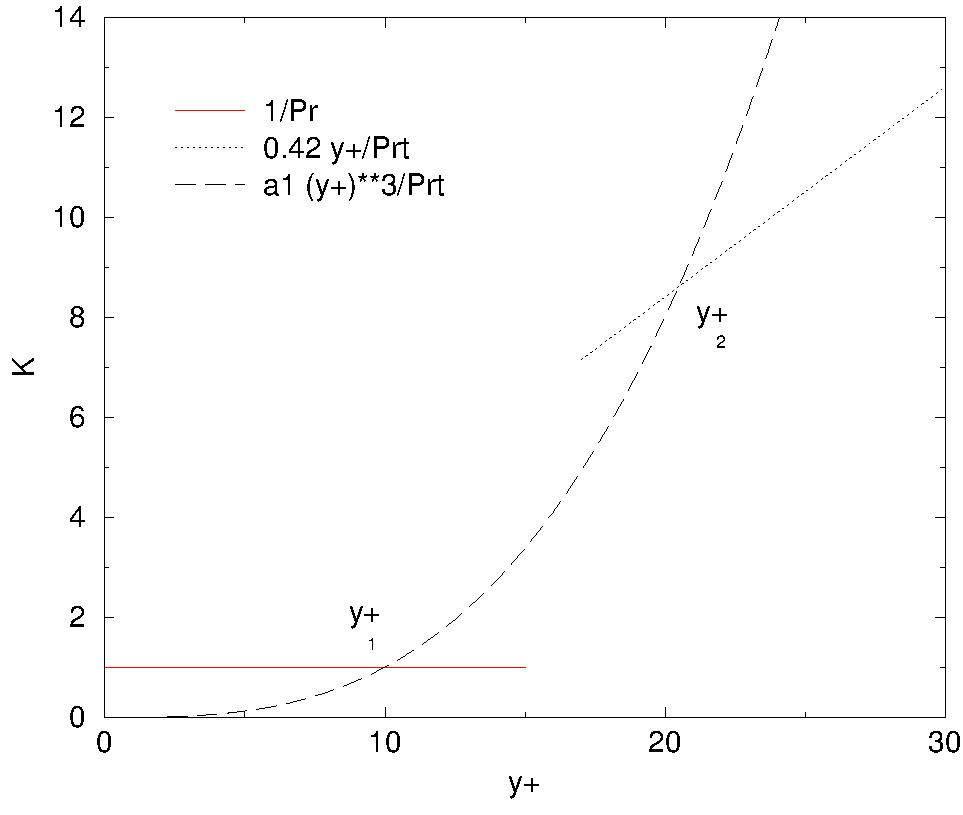
\includegraphics[height=8cm]{\repgraphics/clthermique}}
\caption{Courbes $(a+a_t)/\nu$ fonction de $y^+$ obtenues
                       pour $\sigma=1$ et $\sigma_t=1$.}
\end{figure}


Les valeurs de $y^+_1$ et $y^+_2$ sont obtenues en calculant les
points d'intersection des lois de variation utilis\'ees pour $\mathcal{K}$.


L'existence de la zone interm\'ediaire d\'epend en particulier
des valeurs de $\sigma$.
Consid\'erons tout d'abord les cas pour lesquels $\sigma$ n'est pas
n\'egligeable devant 1. En pratique on consid�re $\sigma > 0,1$
(c'est le cas rencontr\'e couramment lorsque le scalaire $f$ repr\'esente
la temp\'erature de l'air ou de l'eau dans les conditions normales de
temp\'erature et de pression). On suppose que l'on peut n\'egliger
$\displaystyle\frac{1}{\sigma}$ devant
$\displaystyle\frac{a_1 (y^+)^3}{\sigma_t}$ dans la zone interm\'ediaire.
On obtient alors~:
\begin{equation}
  y^+_1 =\left(\displaystyle\frac{1000}{\sigma}\right)^\frac{1}{3} \qquad\qquad
  y^+_2 = \sqrt{\displaystyle\frac{1000\kappa}{\sigma_t}}
\end{equation}
On int\`egre l'�quation adimensionnelle~(\ref{Base_Clptur_Eq_Flux_scalaire_adim})
sous la m\^eme hypoth\`ese et on obtient alors la loi donnant $f^+$~:
\begin{equation}
\left\{
\begin{array}{ll}
f^+ = \sigma \,y^+ & \text{pour } y^+ < y^+_1 \\
f^+ = a_2 -\displaystyle\frac{\sigma_t}{2\,a_1\,(y^+)^2}& \text{pour } y_1^+ \leqslant y^+ < y_2^+ \\
f^+ = \displaystyle\frac{\sigma_t}{\kappa}\,ln(y^+)+a_3& \text{pour } y^+_2 \leqslant y^+\\
\end{array}
\right.
\end{equation}
o\`u $a_2$ et $a_3$ sont des constantes d'int\'egration,
choisies de mani\`ere \`a assurer la
continuit\'e du profil de $f^+$~:
\begin{equation}
a_2=15\sigma^{\frac{2}{3}}\qquad\qquad
a_3=15\sigma^{\frac{2}{3}}-\displaystyle\frac{\sigma_t}{2\kappa}
\left(1+
ln\left(\displaystyle\frac{1000\kappa}{\sigma_t}\right)\right)
\end{equation}


Pla\c cons nous \`a  pr\'esent dans le cas o\`u $\sigma$ est tr\`es petit
devant 1. En pratique on suppose $\sigma \leqslant 0,1$ (c'est par exemple
le cas des m\'etaux liquides pour lesquels  la conduction thermique
s'\'etend tr�s loin et qui pr\'esentent des valeurs du nombre de Prandtl de
l'ordre de 0,01). La couche interm\'ediaire dispara\^\i t alors et l'abscisse
du raccord entre la loi utilis\'ee en proche paroi et celle utilis\'ee loin
de la paroi est donn\'ee par~:
\begin{equation}
y^+_0= \displaystyle\frac{\sigma_t}{\kappa\sigma}
\end{equation}
On int\`egre l'�quation adimensionnelle~(\ref{Base_Clptur_Eq_Flux_scalaire_adim})
sous la m\^eme hypoth\`ese et on obtient alors la loi donnant $f^+$~:
\begin{equation}
\left\{
\begin{array}{ll}
f^+ = \sigma \,y^+ & \text{pour } y^+ \leqslant y^+_0 \\
f^+ = \displaystyle\frac{\sigma_t}{\kappa}\,
        ln\left(\displaystyle\frac{y^+}{y^+_0}\right)+\sigma \,y^+_0
                   & \text{pour } y^+_0 < y^+\\
\end{array}
\right.
\end{equation}


\newpage
Ainsi donc, pour r\'esumer, le calcul de $h_b$
\begin{equation}
h_b=\displaystyle\frac{\phi_b}{f_{b,ext}-f_{I'}}=\frac{\rho\,C\,u_k}{f^+_{I'}}
\end{equation}
est r\'ealis\'e en d\'eterminant $f^+_{I'}$ \`a partir de $y^+=y^+_{I'}$
selon  les lois suivantes.

Si $\sigma\leqslant 0,1$, on utilise un mod\`ele \`a deux couches~:
\begin{equation}
\left\{
\begin{array}{ll}
f^+ = \sigma \,y^+ & \text{pour } y^+ \leqslant y^+_0 \\
f^+ = \displaystyle\frac{\sigma_t}{\kappa}\,
        ln\left(\displaystyle\frac{y^+}{y^+_0}\right)+\sigma \,y^+_0
                   & \text{pour } y^+_0 < y^+\\
\end{array}
\right.
\end{equation}
avec
\begin{equation}
y^+_0= \displaystyle\frac{\sigma_t}{\kappa\sigma}
\end{equation}


Si $\sigma > 0,1$, on utilise un mod\`ele \`a trois couches~:
\begin{equation}
\left\{
\begin{array}{ll}
f^+ = \sigma \,y^+ & \text{pour } y^+ < y^+_1 \\
f^+ = a_2 -\displaystyle\frac{\sigma_t}{2\,a_1\,(y^+)^2}& \text{pour } y_1^+ \leqslant y^+ < y_2^+ \\
f^+ = \displaystyle\frac{\sigma_t}{\kappa}\,ln(y^+)+a_3& \text{pour } y^+_2 \leqslant y^+\\
\end{array}
\right.
\end{equation}
avec
\begin{equation}
  y^+_1 =\left(\displaystyle\frac{1000}{\sigma}\right)^\frac{1}{3} \qquad\qquad
  y^+_2 = \sqrt{\displaystyle\frac{1000\kappa}{\sigma_t}}
\end{equation}
et
\begin{equation}
a_2=15\sigma^{\frac{2}{3}}\qquad\qquad
a_3=15\sigma^{\frac{2}{3}}-\displaystyle\frac{\sigma_t}{2\kappa}
\left(1+
ln\left(\displaystyle\frac{1000\kappa}{\sigma_t}\right)\right)
\end{equation}

%%%%%%%%%%%%%%%%%%%%%%%%%%%%%%%%%%
%%%%%%%%%%%%%%%%%%%%%%%%%%%%%%%%%%
\section{Mise en \oe uvre}
%%%%%%%%%%%%%%%%%%%%%%%%%%%%%%%%%%
%%%%%%%%%%%%%%%%%%%%%%%%%%%%%%%%%%

%\etape{Mode de prescription des conditions aux limites\vspace{0,3cm}}
%%%%%%%%%%%%%%%%%%%%%%%%%%%%%%%%%%%%%%%%%%%%%%%%%%%%%%%%%%%%%%%%%%%%
On traite ici les variables \var{IVAR} sur les faces \var{IFAC}
telles que \var{ICODCL(IFAC,IVAR)}=5.

La vitesse de d\'efilement (\'eventuellement nulle) de la paroi est tout d'abord
projet\'ee dans le plan tangent \`a la paroi. Ses trois composantes dans le
rep\`ere de calcul sont stock\'ees dans les
tableaux\\  \var{RCODCL(IFAC,IUIPH,1),RCODCL(IFAC,IVIPH,1)RCODCL(IFAC,IWIPH,1)}.

On d\'etermine ensuite le
rep\`ere local $\hat{\mathcal R}$. Pour chaque face, il est disponible dans les
vecteurs $\vect{\tau}$ \var{(TX, TY, TZ)}, $\vect{\tilde{n}}$ \var{(-RNX, -RNY,
-RNZ)}, et $\vect{b}$ \var{(T2X, -T2Y,-T2Z)}. Il faut noter que le troisi\`eme
vecteur n'est n\'ecessaire (et n'est donc calcul\'e) que lorsque le mod\`ele de
turbulence $R_{ij}-\varepsilon$ est utilis\'e (pour la projection du tenseur
d'ordre deux). Par ailleurs, si la norme de la vitesse
tangentielle est inf\'erieure \`a la valeur arbitraire \var{EPZERO}
($10^{-12}$), l'indicateur \var{TXN0} est positionn\'e \`a 0 (il vaut 1 sinon)
et le vecteur $\vect{\tau}$ est pris
\begin{itemize}
\item [-] arbitraire, dans le plan perpendiculaire \`a $\vect{\tilde{n}}$ en
$R_{ij}-\varepsilon$  (on utilise les composantes de $\vect{\tilde{n}}$ pour
construire  $\vect{\tau}$~; si  $\vect{\tilde{n}}$ est identiquement nul, le
code s'arr\^ete)~;
\item [-] identiquement nul sinon.
\end{itemize}

Une fois le rep\`ere local d\'etermin\'e, le sous-programme \fort{clca66} est
appel\'e avec\footnote{\var{CLSYME} = 0 permet de sp\'ecifier qu'on
traite les conditions de paroi et non des conditions de sym\'etrie. On pourra se
reporter \`a \var{CLSYVT} pour les d\'etails de \fort{clca66}.} \var{CLSYME} =0
si le mod\`ele $R_{ij}-\varepsilon$ est activ\'e, afin de calculer la
matrice \var{ALPHA} qui permettra, \`a partir des valeurs du tenseur de Reynolds
au points $I'$, de calculer les valeurs \`a imposer aux faces de bord.

On calcule ensuite les vitesses de frottement qui sont stock\'ees dans
\var{UET} ($=u^*$) et dans \var{UK} ($=u_k$). Le sous-programme \fort{causta}
 permet de calculer la vitesse de
frottement pour le mod\`ele \`a une \'echelle
de vitesse (\var{IDEUCH}=0). Pour le mod\`ele \`a deux \'echelles
(\var{IDEUCH}=1), le calcul (plus simple) de \var{UET} et de \var{UK} est fait directement
dans \fort{clptur}. Le sous-programme utilisateur \fort{usruet} permet alors de
donner la main \`a l'utilisateur qui souhaiterait  modifier les \'echelles de
vitesses (prise en compte d'une paroi rugueuse, ou de variantes de
la loi logarithmique par exemple).

Dans le cas ou le mod\`ele \`a une \'echelle de vitesse est actif, on impose
\var{UK=UET} afin de conserver la coh\'erence du codage dans la suite du
sous-programme. N\'eanmoins, dans le cas o\`u on se trouve dans la sous-couche visqueuse, on force \var{UK=0} ce qui
permettra d'obtenir une valeur nulle pour $k$ et un flux nul pour $\varepsilon$
(la valeur \var{UET} n'est pas utilis\'ee, car la condition sur la vitesse
devient une condition d'adh\'erence et les tensions de Reynolds sont annul\'ees).
Si l'on se trouve dans la sous-couche visqueuse, on recalcule \var{UET}
(et \var{YPLUS} si l'on est \`a une \'echelle de vitesse) car l'\'evaluation
pr\'ec\'edente a \'et\'e faite avec l'hypoth\`ese que l'on \'etait en zone
logarithmique.

Les conditions aux limites pour la vitesse sont ensuite compl\'et\'ees.
\begin{itemize}

\item [-] En $k-\varepsilon$, on affecte, pour les trois composantes de vitesse
respectivement, \`a $$\var{COEFA(IFAC,ICLUF)}, \var{COEFA(IFAC,ICLVF)} \,\text{ et
}\,\var{COEFA(IFAC,ICLWF)}$$ les coefficients $A_{flux}$
issus de l'analyse relative \`a la contrainte tangentielle.\\
 De m\^eme, les coefficients $B_{flux}$ sont affect\'es \`a
$$\var{COEFB(IFAC,ICLUF)}, \var{COEFB(IFAC,ICLVF)} \,\text{ et
}\,\var{COEFB(IFAC,ICLWF)}.$$ Les conditions aux limites
issues de l'analyse portant directement sur le gradient de vitesse $A_{grad}$ et
$B_{grad}$ sont affect\'ees \`a  $$\var{COEFA(IFAC,ICLU)},
\var{COEFA(IFAC,ICLV)}, \var{COEFA(IFAC,ICLW)}$$ et
$$\var{COEFB(IFAC,ICLU)}, \var{COEFB(IFAC,ICLV)}, \var{COEFB(IFAC,ICLW)}.$$

\item [-] Lorsque la vitesse tangentielle en $I'$ est inf\'erieure \`a
\var{EPZERO}, l'indicateur \var{TXN0} est annul\'e (sinon,  \var{TXN0} vaut 1).
De m\^eme, quand la valeur de
$y^+$ est inf\'erieure ou \'egale \`a $10,88$, l'indicateur
\var{UNTURB} est positionn\'e \`a 0 (sinon, il vaut 1). Ces deux indicateurs sont utilis\'es
pour annuler les coefficients $A$ et imposer des conditions d'adh\'erence.

\item [-] la vitesse de d\'efilement de la paroi est prise en compte dans les
conditions aux limites (coefficients \var{COEFA}).

\end{itemize}

Les conditions sur les grandeurs turbulentes sont ensuite compl\'et\'ees.
Une pr\'ecision est n\'ecessaire pour le tenseur de Reynolds en
$R_{ij}-\varepsilon$. En notation tensorielle on souhaite obtenir
$\tens{R}_F = E_{loglo}\,\hat{\tens{R}}_F\,E^t_{loglo}$, o\`u
$\hat{\tens{R}}_F$ est le tenseur des contraintes \`a imposer dans le rep\`ere
de paroi local et $E_{loglo}$ la matrice de passage. Le tenseur dans le rep\`ere
local est d\'efini par les conditions aux limites pr\'ecis\'ees plus haut,
soit $\hat{\tens{R}}_F=\hat{\tens{R}}^{B=1}_F$, avec \footnote{Le param\`etre
$B$ permet d'annuler formellement deux termes si besoin.}~:
\begin{equation}
\hat{\tens{R}}^B_{F}=\left[\begin{array}{lll}
\hat{R}_{\tau\tau,I'}&-Bu^*u_k                       &0\\
-Bu^*u_k             &\hat{R}_{\tilde{n}\tilde{n},I'}&0\\
0                    &0                              &\hat{R}_{bb,I'}
\end{array}\right]
\end{equation}

Le tenseur de Reynolds est cependant stock\'e sous forme d'un vecteur de 6
composantes (aux points $I'$ relatifs aux faces de bord, ces valeurs sont
port\'ees par \var{RIJIPB(IFAC,II)}, avec \var{IFAC} le num\'ero de la face et
\var{II} le num\'ero de la contrainte, de 1 \`a 6 pour d\'esigner dans l'ordre
$R_{11},R_{22}, R_{33}$ et
$R_{12}, R_{13}, R_{23}$. La table \var{ALPHA} de dimension
$6\times 6$ calcul\'ee par \fort{clca66} permet d'effectuer les calculs de
changement de rep\`ere necessaires et d'obtenir les valeurs
$\hat{\tens{R}}^{B=0}_F$ \`a partir des valeurs contenues dans
\var{RIJIPB(IFAC,II)}.
Ainsi,
\begin{itemize}
\item[-] pour chaque tension de Reynolds \var{ISOU},
dans le cas de conditions aux limites explicites (\var{ICLPTR}=0), on affecte \`a
\var{COEFA(IFAC,ISOU)}  la valeur
$\tens{R}^{B=1}_F$ correspondante  obtenue en calculant d'abord
$\tens{R}^{B=0}_F$ par
$\sum_{II=1,6}$\var{ALPHA(ISOU,II)*RIJIPB(IFAC,II)}, puis en y ajoutant la
quantit\'e en facteur de B dans l'expression formelle
de la somme sus-nomm\'ee, afin d'obtenir la valeur compl\`ete de
$\tens{R}^{B=1}_F$.
Les conditions aux limites \'etant explicites, \var{COEFB} prend la valeur 0.
\item[-] dans le cas de conditions aux limites semi-implicites (\var{ICLPTR}=1),
pour chaque tension de Reynolds \var{ISOU},
on affecte au tableau \var{COEFA(IFAC,ISOU)} la valeur
$\tens{R}^{B=1}_F$ correspondante diminu\'ee des termes d\'ependants de
\var{RIJIPB(IFAC,ISOU)} qui seront implicit\'es. Cette valeur est obtenue en
calculant d'abord \\
$\sum_{II=1,6|II\neq ISOU}$\var{ALPHA(ISOU,II)*RIJIPB(IFAC,II)},
puis en ajoutant la quantit\'e en facteur de B afin d'obtenir la valeur de $\tens{R}^{B=1}_F$ diminu\'ee
du terme\\ \var{ALPHA(ISOU,ISOU) RIJIPB(IFAC,ISOU)}. On affecte ensuite la valeur
\var{ALPHA(ISOU,ISOU)} \`a \var{COEFB} (partie implicite des
conditions aux limites)\footnote{L'implicitation ne concerne pas la contrainte
tangentielle issue des vitesses de frottement et n'est donc pas totale.}.
\end{itemize}

Les conditions aux limites pour les scalaires sont ensuite compl\'et\'ees. Les
coefficients \var{COEFA} et \var{COEFB} sont simplement renseign\'es en
utilisant les conditions aux limites d\'ecrites pr\'ec\'edemment. La seule
difficult\'e consiste \`a g\'erer correctement les diff\'erentes grandeurs
permettant de
calculer le coefficient d'\'echange $h_b$ sans erreur.

L'indicateur \var{ISCSTH} sert, pour chaque {\it VarScalaires} \`a indiquer
quelle valeur de $C$ utiliser
au moment du traitement des conditions aux limites. Ainsi, pour \var{ISCSTH}=1,
la variable doit \^etre trait\'ee comme une temp\'erature, avec $C=C_p$. Pour
\var{ISCSTH}=0 ou 2, la variable doit \^etre trait\'ee comme un scalaire passif
ou une enthalpie respectivement, avec  $C=1$ (constante sans dimension) dans les
deux cas. Pour \var{ISCSTH}=3, la variable est l'�nergie r�solue dans le cadre
du module compressible (cf. \fort{cfxtcl}). On a alors $C=1$.

Par ailleurs, une valeur strictement positive de l'entier \var{IPCCP}
indique que  $C_p$ est variable en espace
et disponible dans le tableau \var{PROPCE(IEL,IPCCP )} (renseign\'e dans
\var{USPHYV}). Lorsque \var{IPCCP} est
nul, $C_p$ est constant et disponible sous
forme du  r\'eel \var{CP0(IPHAS)}.

L'indicateur \var{IHCP} permet de rassembler ces informations~:
\begin{itemize}
\item [-] \var{IHCP} = 0 : \var{CPP} = $C=1$
\item [-] \var{IHCP} = 1 : \var{CPP} = $C=C_p$ uniforme en espace
\item [-] \var{IHCP} = 2 : \var{CPP} = $C=C_p$ variable en espace
\end{itemize}

Pour la {\it VarScalaire} \var{LL}, l'indicateur \var{IVISLS(LL)}
permet \'egalement de rep\'erer si $\displaystyle\frac{\alpha_m}{C}$
est variable en espace et disponible dans le tableau \var{PROPCE(IEL,IPCVSL)}
(\var{IVISLS} $> 0$) ou uniforme en espace et disponible sous forme du r\'eel
\var{VISLS0(LL)} (\var{IVISLS} $= 0$). On pose \var{RKL}$ =
\displaystyle\frac{\alpha_m}{C}$

Le nombre de Prandtl local est alors calcul\'e \var{PRDTL} $ =
\displaystyle\frac{\mu}{\alpha_m/C}$ ($\mu$ est la viscosit\'e dynamique mol\'eculaire
disponible dans  \var{VISCLC}).

Le coefficient $h_{int}=\displaystyle\frac{\alpha}{\overline{I'F}}$  est ensuite
d\'etermin\'e et conserv\'e
dans \var{HINT}.

Lorsqu'un mod\`ele de turbulence est activ\'e,
le sous-programme \var{HTURBP} permet le calcul de \var{HFLUI} $ =
Pr\displaystyle\frac{y^+}{T^+}$ (ou \var{HFLUI}~$ = 1$ dans la sous-couche visqueuse),
que l'on multiplie imm\'ediatement par \var{CPP*RKL/DISTBF}$ =
\displaystyle\frac{\alpha_m}{\overline{I'F}}$ pour obtenir \var{HFLUI} $ = h_b =
\displaystyle\frac{\rho C u_k}{T^+}$ (ou \var{HFLUI} $ = h_b = \displaystyle\frac{\alpha_m}{\overline{I'F}}$ dans la
sous-couche visqueuse).  Si le calcul est r\'ealis\'e en laminaire, on a
simplement \var{HFLUI} = \var{HINT} ($ = h_b = h_{int}=\displaystyle\frac{\alpha}{\overline{I'F}}$)

Dans les cas o\`u l'on souhaite stocker le coefficient d'\'echange (couplage
avec SYRTHES), \var{HFLUI} est conserv\'e dans le tableau \var{HBORD}.
Dans les cas o\`u l'on utilise le module de rayonnement, \var{HFLUI} est
stock\'e  dans le tableau de travail \var{RA(IHCONV)}.

On dispose alors de tous les \'elements pour calculer les coefficients $A$ et
$B$ (\var{COEFA} et \var{COEFB}) relatif \`a la variable trait\'ee. Noter pour
terminer les
correspondances suivantes qui permettent de rapprocher le code source de la
relation (\ref{Base_Clptur_eq_fbint_clptur})~: \var{HEXT} $ = h_{imp,ext}$, \var{PIMP} $ = f_{imp,ext}$,
\var{HREDUI} $ = h_r$, \var{HINT} $ = h_{int}$,  \var{HFLUI} $ = h_b$.





\newpage
%%%%%%%%%%%%%%%%%%%%%%%%%%%%%%%%%%
%%%%%%%%%%%%%%%%%%%%%%%%%%%%%%%%%%
\section{Points \`a traiter}
%%%%%%%%%%%%%%%%%%%%%%%%%%%%%%%%%%
%%%%%%%%%%%%%%%%%%%%%%%%%%%%%%%%%%


L'utilisation de \var{HFLUI/CPP} lorsque \var{ISCSTH} vaut 2 (cas du
rayonnement) est \`a v\'erifier (\var{CPP} vaut en effet 1 dans ce cas).

Les conditions aux limites pour la vitesse sont bas\'ees sur des
consid\'erations portant sur un seul terme de la contrainte tangentielle
$(\mu_I+\mu_{t,I})(\ggrad{\vect{u}})\,\vect{n}$ sans aucune prise en compte du
gradient transpos\'e.

Pour \'etablir les  conditions aux limites portant sur la vitesse en
$k-\varepsilon$ \`a partir des consid\'erations sur la contrainte, on introduit
une projection sur le plan tangent \`a la paroi et on impose arbitrairement
une vitesse normale nulle.

Les hypoth\`eses faites pour \'etablir les formules des diff\'erents types de
conditions aux limites (dissipation, vitesses) sont bas\'ees sur des
hypoth\`eses de maillage orthogonal en paroi. Elles sont \'etendues sans
pr\'ecaution aux maillages non orthogonaux.

La loi de paroi \`a une \'echelle de vitesse (\fort{causta}) n\'ecessite la
r\'esolution d'une \'equation au moyen d'un algorithme de Newton.
Le co\^ut de ce dernier est faible. On peut \'egalement utiliser
une loi en puissance $1/7$ (Werner et Wengle) qui produit,  dans la zone
logarithmique,  des r\'esultats aussi pr\'ecis que la loi logarithmique
et permet des r\'esolutions analytiques (option choisie pour la version LES).
Attention n\'eanmoins, car avec cette loi, l'intersection avec la loi
lin\'eaire est l\'eg\`erement diff\'erente, ce qui requiert donc des
adaptations (intersection vers 11,81 au lieu de 10,88 pour la loi choisie ici
$U^+=8,3\,(y^+)^\frac{1}{7}$).

Les valeurs de toutes les propri\'etes physiques sont prises au centre des
cellules, sans reconstruction. Il ne s'agit pas de modifier forc\'ement cette
approche, mais il serait bon de garder ce fait pr\'esent \`a l'esprit.

%
%
%
%Pb de continuite si YPLULI.NE.10.88
%
% Le mode de r\'esolution permettant d'obtenir $u^*$ est particulier. Avec le
%mod\`ele \`a une \'echelle de vitesse, on \'evalue
%tout d'abord la vitesse de frottement $u^*$ issue de la loi logarithmique. On
%pose $u_k=u^*$, puis on calcule la valeur de $y^+$.  Avec le
%mod\`ele \`a deux \'echelles, on calcule tout d'abord $u_k$, on en d\'eduit
%$y^+$ puis $u^*$. Dans les deux cas, si
%$y^+\leqslant y^+_{lim}=\displaystyle\frac{2}{\kappa}$, on applique une condition
%d'adh\'erence (vitesse impos\'ee nulle \`a la paroi, \'energie turbulente et
%tensions de Reynolds impos\'ees nulles, flux nul pour la dissipation).
%Il serait bon de v\'erifier que cette m\'ethode, qui utilise une loi
%logarithmique jusqu'\`a de tr\`es petites
%valeurs de $y^+$, ne conduit pas \`a des valeurs trop faibles de la
%vitesse de frottement lorsqu'on s'approche de la paroi ($y^+ \leqslant 10$).
%La figure \ref{Base_Clptur_fig_loi_log_clptur} propose une illustration~: supposons qu'en un
%point on obtienne, avec la m\'ethode actuelle, $u+\approx 8,6$ et
%$y^+\approx 4,3$. On en d\'eduit alors que la vitesse de frottement est
%$u^*\approx 1$ (courbe logarithmique en trait plein (noire) repr\'esentant
%$ln(y^+)/0,42+5,2$).
%Toutes choses \'egales par ailleurs (ce qui constitue une
%hypoth\`ese en soi), avec une m\'ethode prenant en compte une loi lin\'eaire en
%dessous de $y^+\approx 10$, on aurait obtenu $u^*\approx 2$
%(courbe lin\'eaire en trait plein (rouge) repr\'esentant $2y^+$). Bien
%entendu, cette analyse est relativement na\"\i ve et ne prend pas en compte le
%caract\`ere implicite des r\'esolutions ainsi que le fait qu'il est d'ordinaire
%peu recommand\'e de placer la premi\`ere maille \`a des valeurs aussi faibles de
%$y^+$ avec les mod\`eles de type haut Reynolds.
%
%\begin{figure}[h]
%\centerline{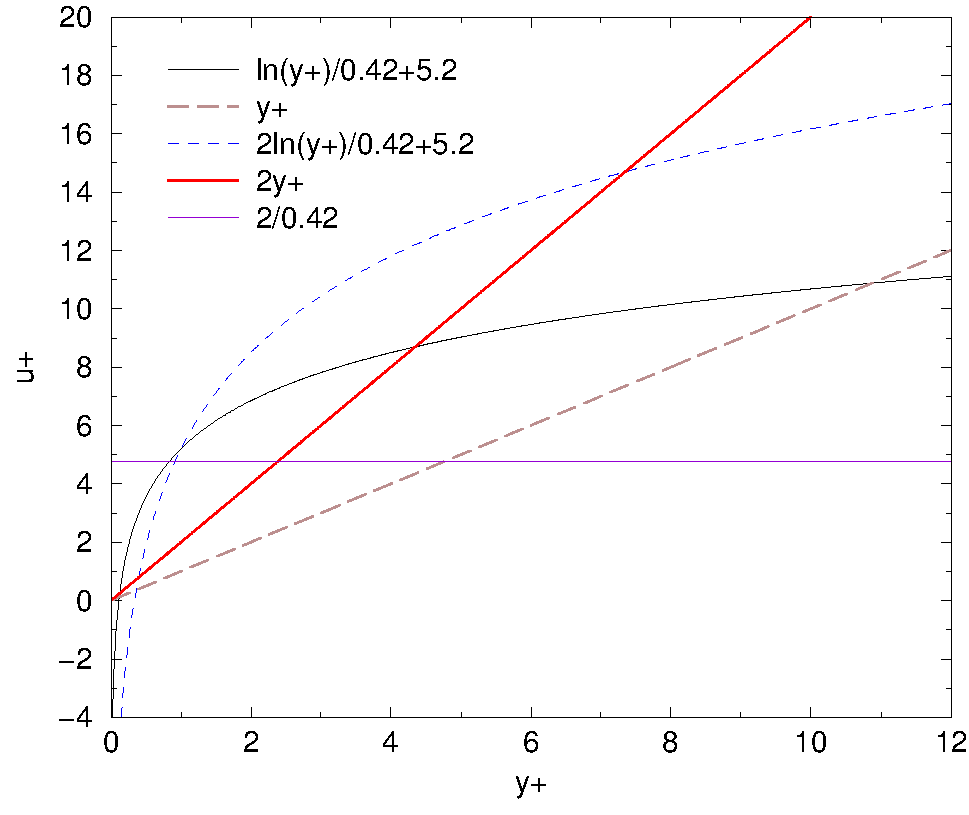
\includegraphics[height=7cm]{\repgraphics/loilog}}
%\caption{\label{Base_Clptur_fig_loi_log_clptur}D\'etermination de $y^+$.}
%\end{figure}



% Plus d'actualite a priori, mais pistes de reflexion quand meme
%La limitation par valeur minimale de la vitesse dans (\ref{Base_Clptur_eq_ugrad_clptur})
%a \'et\'e corrig\'ee dans la version 1.1.0.q.
%Auparavant, la formulation \'etait susceptible de conduire
%\`a une valeur trop faible du gradient de vitesse et donc de la production
%turbulente en paroi. Elle s'\'ecrivait~:
%\begin{equation}
%u_{\tau,F,grad} =u_{\tau,I'}-\displaystyle\frac{u^*}{\kappa}min\left[max\left(1,
%2\sqrt{\displaystyle\frac{\rho_I\kappa\, u_k I'F}{\mu_{t,I}}
%}-\displaystyle\frac{1}{2}\right),ln\frac{2}{\kappa}+5,2\kappa\right]
%\end{equation}
%La  formulation a \'et\'e modifi\'ee~:
%\begin{equation}\notag
%u_{\tau,F,grad} =max\left(u^*(\frac{1}{\kappa}ln\displaystyle\frac{2}{\kappa}+5,2),
%u_{\tau,I'}-\displaystyle\frac{u^*}{\kappa}\left[max\left(1,
%2\sqrt{\displaystyle\frac{\rho_I\kappa\, u_k I'F}{\mu_{t,I}}
%}-\displaystyle\frac{1}{2}\right)\right]\right)
%\end{equation}
%Elle a \'et\'e adopt\'ee apr\`es des tests sur des
%configurations de validation (canal, marche descendante,  jet impactant, dune,
%echo, rra) qui n'ont montr\'e aucune influence de la modification.
%\`A partir de la version 1.1.0.t, on a utilis\'e la valeur
%$y^+_\text{lim}=10,88$ et non plus $\frac{2}{\kappa}$ pour caract\'eriser le
%passage de la loi lin\'eaire \`a la loi logarithmique et la
%relation a donc \'et\'e modifi\'ee comme suit~:
%\begin{equation}\notag
%u_{\tau,F,grad} =max\left(u^*(\frac{1}{\kappa}ln(y^+_\text{lim})+5,2),
%u_{\tau,I'}-\displaystyle\frac{u^*}{\kappa}\left[max\left(1,
%2\sqrt{\displaystyle\frac{\rho_I\kappa\, u_k I'F}{\mu_{t,I}}
%}-\displaystyle\frac{1}{2}\right)\right]\right)
%\end{equation}
%Comme, pour des $y^+$ inf\'erieurs \`a $y^+_\text{lim}$, on applique une
%condition d'adh\'erence, cette approche n'est pas continue au voisinage de
%$y^+_\text{lim}$. Il serait utile de se pencher sur la question.
%Il faut cependant garder \`a l'esprit que la condition
%de Dirichlet pour $k$ est prise nulle quand  $y^+$ est inf\'erieur \`a
%$y^+_\text{lim}$, ce qui tend \'egalement \`a annuler la production,
%quelle que soit la condition \`a la limite utilis\'ee pour la vitesse.

Pour la loi thermique avec des nombres de Prandtl tr\`es petits devant
l'unit\'e, Arpaci et Larsen sugg\`erent de prendre $y_0^+ \simeq 5/Pr$
(en s'appuyant sur des donn\'ees exp\'erimentales) plut\^ot que
$Pr_t/(Pr\,\kappa)$ (valeur adopt\'ee actuellement et
issue de l'intersection analytique des lois
lin\'eaire et logarithmique consid\'er\'ees). Il faudrait se pencher sur
la question.
